\chapter{Introduction}

\subsection{The ALICE experiment}
The ALICE experiment is a collaborative experiment of approximate 1800 persons from 176 institutes in 41 countries. The collaborative work of this scientific and technical community is largely distributed over the planet and covering it from UTC-8 till UTC+9. The experiment is taking data and producing physics results since 2009. During the Long Shutdown in 2019 and 2020 a major upgrade will be done. 

\subsection{The ALICE upgrade}
During the Long Shutdown 2 ALICE will be upgraded. The upgrade will be done on many subsystems:
\begin{description}
  \item[ITS] A new Inner Tracking System will be installed. This new system will have an improved pointing precision. It will also be made of lesser material than before and become the thinnest tracker at the LHC.
  \item[TPC] The Time Projection Chamber will get new GEM technology for the read out chambers. The readout will be continuous and it will use faster readout electronics.
  \item[CTP] A new Central Trigger Processor will be installed.
  \item[DAQ] A brand new Data Acquisition system will be installed.
  \item[HLT] A new High Level Trigger will be installed.
  \item[MFT] In the Muon Forward Tracker a new SI tracker will be installed. The MUON pointing precision will be improved.
  \item[MUON ARM] The MUON ARM will get new continuous readout electronics.
  \item[FIT] There will be new Trigger detectors installed.
  \item[TOF] The TOF will be readout faster.
  \item[TRD] The TRD will be readout faster.
  \item[ZDC] The ZDC will be readout faster.
\end{description}

\begin{figure}[h]
  \begin{center}
    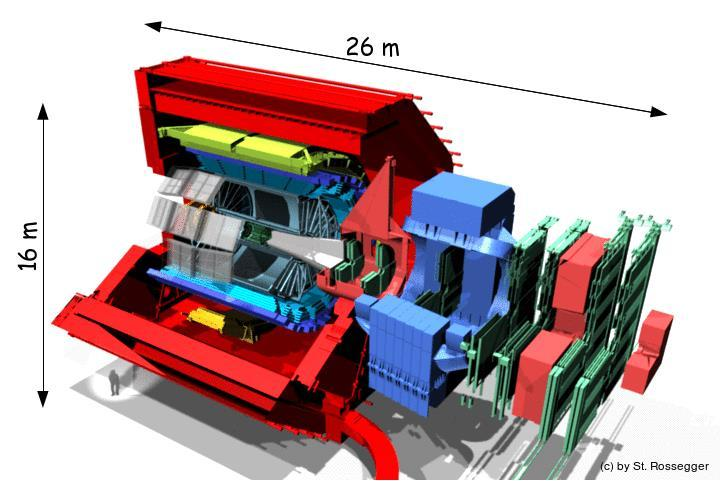
\includegraphics[scale=0.4]{alice_upgrade.jpg}
    \caption{An overview of ALICE}
    \label{fig:overview}
  \end{center}
\end{figure}
After the Long Shutdown 2 the LHC produce Pb–Pb collisions at up to $L = 6.10^{27} cm^{-2} s^{-1}$. This results in an interaction rate of 50kHz. During Run 3 (2021-2023) pp collisions will be done at 14 TeV and Pb-Pb collisions at 5.5 TeV. In 2023 no Pb-Pb collisions are scheduled. After Long Shutdown 3 (2024-2026) the same schedule will be realised except for 2028 when p-Pb will be run at 8.8 TeV.

The 50 kHz rate for collisions produces about 100 times more data than was produced in 2010. This will give the physicists the opportunity to detect very rare processes with very small signal over background ratio. Because the triggering techniques are very inefficient if not impossible support for continuous read-out is developed. Therefore a new computing system, $O^2$, is created. It will read-out the data of all interactions. Compress these data intelligently by online reconstruction. The system will be one common online-offline computing system.

Unmodified raw data of all interactions shipped from detector to online farm in triggerless continuous mode. This will amount to 3.4 TB/s. Then a baseline correction and zero suppression will take place. The data volume will be reduced by zero cluster finder. No event is discarded. The average compression factor is 6.6. Then 500 GB/s will be shipped. A data volume reduction is done by online tracking. Only reconstructed data will be send to data storage. The average compression factor is 5.5. From here 90 GB/s will be transported. In the data Storage 1 year of compressed data will be kept. From this storage facility 20 GB/s will be transported to tier 0 and tier 1. The events will also be reconstructed for final calibration.

From the detector electronics 8500 GBTs links will send signals to the 270 FLPs. These will use hardware acceleration using FPGAs. A switching network will distribute this data to 1500 EPNs. These processing nodes use GPUs for hardware acceleration. The EPNs use a switching network to send the data to the storage. This storage can write at 170 GB/s and read at 270 GB/s. The capacity for storage is 60 PB.

To manage the $O^2$ update several work packages are created:
\begin{description}
  \item[WP 1] Data Model
  \item[WP 2] Data Flow and System Simulation
  \item[WP 3] Common Tools and Software
  \item[WP 4] $O^2$ Software Framework– Common tools and infrastructure
  \item[WP 5] Data distribution and load balancing
  \item[WP 6] Detector readout
  \item[WP 7] Quality Control
  \item[WP 8] Control, Configuration and Monitoring
  \item[WP 9] Event Display
  \item[WP 10] Constant and Calibration DB
  \item[WP 11] ALFA
  \item[WP 12] Simulation
  \item[WP 13] Reconstruction and Calibration
  \item[WP 14] Analysis framework and facility infrastructure
  \item[WP 15] Data Management
  \item[WP 16] Computing Room CR1 (FLP)
  \item[WP 17] Computing Room CR0 (EPN)
\end{description}

\section{Purpose}
The purpose of this Software Requirements Specifications document is to have a central point for all the requirements of the bookkeeping system. It is not written with the goal to have a document with definite and final requirements for this system. During the process of developing this system requirements will be added and modified.

\subsection{Upgrade of the bookkeeping}
ALICE will do a major upgrade in 2019/2020 when the Long Shutdown 2 will be done. During this period the new Online-Offline ($O^2$) computer system will be implemented. This gives an opportunity to upgrade the bookkeeping facility currently in use. The bookkeeping currently consists of two not related systems: the Electronic Logbook and AliMonitor. These systems have been developed since 2009 and evolved gradually during the years. Due to this development process the applications are in some ways a bit confusing, not efficient and overall candidates for improvement, let alone their fusion which seems an improvement in itself. In Section XX a description of the current system is given. It seems to be most sensible to do such an during a Long Shutdown because of the overall break in activities at ALICE. New detectors are being installed, the LHC stops running, etc. An update done during a winter break which is always taking place between half December and March would have been a possibility. Doing such an update during run season does not seem to be appropriate because of the importance of the bookkeeping system for ALICE. It is expected that the next opportunity to replace the current systems is over 10 years. That would take too long for the current systems to exist.

\begin{figure}[h]
  \begin{center}
    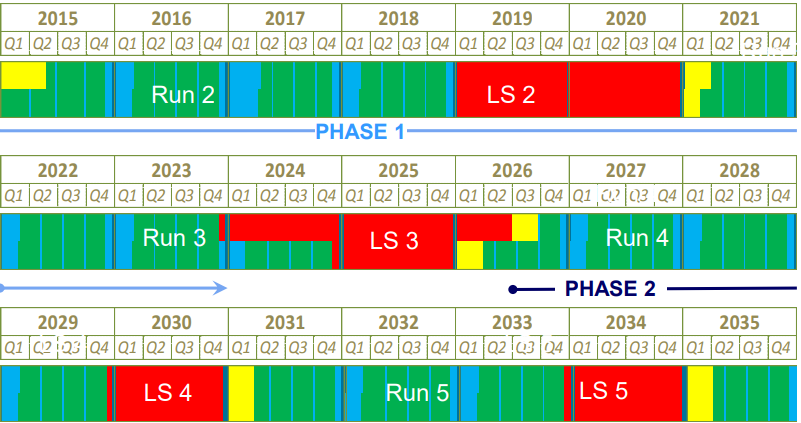
\includegraphics[scale=0.3]{./timetable.png}
    \caption{Time table for the LHC}
    \label{fig:timetable}
  \end{center}
\end{figure}

The motivation to do an upgrade is threefold. First it makes sense to unify the two systems, i.e. the electronic logbook and AliMonitor, now used to bookkeeping for ALICE. In this respect it should be mentioned that some users of AliMonitor themselves use separate systems to store information which arguably should be part of the bookkeeping system, e.g. JIRA. Secondly, although in the years of its existing a lot of features were added, this is not been done anymore since it was clear the system would be replaced. Features which have been mentioned the last few years are only when really needed, implemented. This means that there is a list of features not implemented but still wished for. Lastly, because the system was developed starting around 2009 it is based on relatively old technologies. 

The goal is a bookkeeping system which is responsive to different media used and has a unified look and feel. It should be compatible to the current system and accessible from inside and outside of CERN. The authorisation and authentification should be based on the central systems as made available by CERN. It should be supported as long as it is in use by ALICE.

There are several challenges for the update of the bookkeeping system. The bookkeeping system is critical to the ALICE operations. It is critical because without proper bookkeeping of the data, i.e. bookkeeping the metadata referring to the physics data produced by ALICE, the data itself, i.e. the data produced by the detectors, becomes useless. The workflows which should be registered in the system are quite complex. Because the AUAS is a newcomer to the High Energy Physics community a lot has to be learned about vocabulary and jargon. The schedule for the project is also a challenge. At the end of next year (2018) a (small) part of the system has to be delivered while the whole system should be in production in 2021. Another difficulty for the project is found in the migration from the existing to the new tool. A part of the bookkeeping system concerns the off line activity for recovering data and quality control. This work will not stop during the Long Shutdown 2 and for this work to be done a continuous use of the system will take place. Lastly, support for the system will have to be done until 2029.

During Run 1 and 2 a lot of experience concerning the use of the bookkeeping system is accumulated. Developers of the new system have the opportunity to elicit the experience of the past users and use this to their advantage. Modern technologies should make it more easy to develop a bookkeeping system. Because the AUAS is the task owner to create the bookkeeping system it is expected this should generate a lot of energy to make it happen.

\subsection{Vision}
Provide unified bookkeeping experience for operations, run catalogue and management.

\subsection{Needs}
Access in a single place all metadata related with operational activities. Keep historical record of used configurations, statistics and data quality. Produce reports for operational teams and management. 

\subsection{Product}
Dashboards for run metadata with different levels of detail. Search for data sets that match given criteria. Forms for creating textual log entries. Notifications for interventions, main events and summary reports. API for read/write access to metadata repository. 


\subsection{Business goals}
Adapt to new O2 data model. Consolidate existing ALICE Electronic Logbook and Run Conditions Table in a single product. Refresh used technologies and make the product more future oriented. Integrate gathered experience and introduce missing features. 



\section{Scope of the Bookkeeping System}
The scope of the project to develop the bookkeeping system is restricted to keeping track of the configuration of ALICE, data produced by ALICE, and computations on this data. The bookkeeping system is not a monitoring system for ALICE.

\section{Definitions, Acronyms, and Abbreviations}

\subsection{Log Entry}
A Log Entry is a text message that describe an intervention or an event that happened. It can be generated either by humans (e.g. a shifter enters his/her end-of-shift report) or by machines (e.g. a detector logs some abnormal situation automatically). 

\subsection{Run}
A Run is a unique ID that identifies a synchronous data processing session in the $O^2$ computing system with a specific and well-defined configuration. It normally ranges from a few minutes to tens of hours. It is generated and managed by the $O^2$ system. 

\subsection{LHC Fill}
An LHC Fill is a unique ID that identifies a period of activity in the LHC accelerator. It normally ranges from a few minutes to tens of hours. It is generated and managed by the LHC system and published via DIP protocol. 
 
\begin{table}[h]
\begin{center}
\begin{longtable}{ll}
    ALICE & A Large Ion Collider Experiment\\
    API & Application Programming Interface\\
    DAQ & Data Acquisition subsystem \\
    ID & Identity Document\\
    IEEE & Institute of Electrical and Electronics Engineers\\
     LHC  & Large Hydron Collider\\\
     $O^2$ & Online and Offline\\
     
       & \\
    \end{longtable}
      \caption{Acronyms}
  \label{tab:acronyms}
  \end{center}
  
\end{table}




\section{References}

\section{Overview}
This document is structured according to the IEEE standard 830-1998 Recommended Practice for Software Requirements Specifications.
